\subsection{Examples}

\begin{example2}{Was ist Computertechnik?}\\
  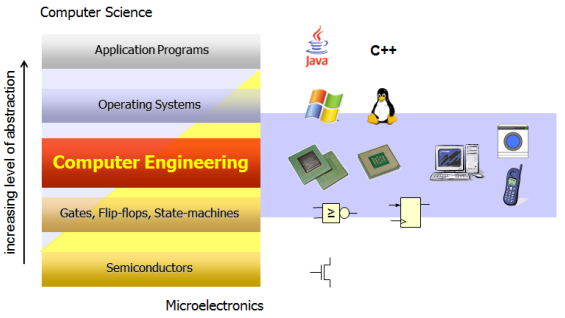
\includegraphics[width=\linewidth]{images/wasistcomputertechniik.png}
\end{example2}

\begin{example2}{Struktur eines Computersystems}\\
Skizzieren Sie die Struktur eines Computersystems:\\
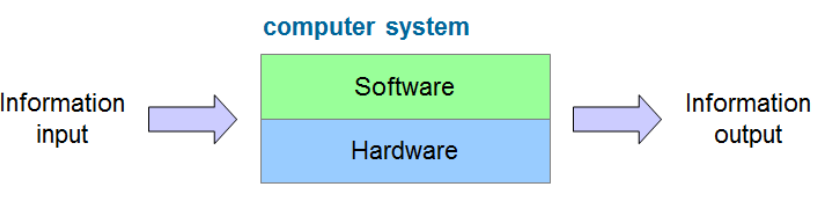
\includegraphics[width=\linewidth]{images/strukturcomputersystem.png}
\end{example2}

\begin{example2}{Komponenten eines Computersystems}\\
Nennen Sie 4 grundlegende Komponenten eines Computersystems und beschreiben Sie die Aufgaben jeder Komponente:
\begin{itemize}
  \item \textbf{CPU (Central Processing Unit)} oder Prozessor: Führt Anweisungen und Daten aus
  \item \textbf{Memory}: Speichert Anweisungen (Instructions) und Daten
  \item \textbf{Input/Output}: Eingabe/Ausgabe Interface zu externen Geräten
  \item \textbf{System Bus}: Elektrische Verbindung von Funktionseinheiten
\end{itemize}
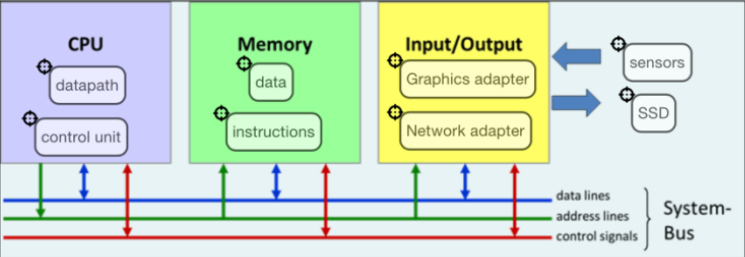
\includegraphics[width=\linewidth]{images/komponentenversion2.png}
\end{example2}



\begin{example2}{Computer System Components}\\
Examples of basic computer system components and their interactions:

\begin{lstlisting}[language=C, style=basesmol]
// Example showing interaction between components
int main(void) {
    int data;            // Uses Memory
    scanf("%d", &data);  // Uses I/O
    data = data * 2;     // Uses CPU/ALU
    printf("%d", data);  // Uses I/O
    return 0;
}
\end{lstlisting}
\end{example2}

\begin{example2}{Steuereinheit einer CPU}\\
Beschreiben Sie die Aufgaben der Steuereinheit einer CPU:\\
Die Steuereinheit liest, interpretiert und führt Anweisungen aus. Sie steuert den Programmablauf und verwaltet den Befehlsablauf.
\end{example2}

\begin{example2}{von Neumann Architecture}\\
Erklären Sie die von Neumann Architektur:\\
\includegraphics[width=\linewidth]{images/vonneumannerklärung.png}
\end{example2}

\begin{example2}{Programmübersetzung}\\
Nennen und erklären Sie die vier Schritte der Programmübersetzung. Welche Output Dateien werden erzeugt?\\
\textbf{Preprocessor:}
\begin{itemize}
  \item Verarbeitet die Preprocessor Statements (z.B. \#include, \#define)
  \item Textprocessing: Ersetzen und Ergänzen von Inhalten
  \item \textbf{Output:} Textfile mit modifiziertem C Source Code (.i)
\end{itemize}
\textbf{Compiler:}
\begin{itemize}
  \item Übersetzt C Code in prozessorspezifische, symbolische Assemblerbefehle
  \item Optimierung (falls aktiviert)
  \item \textbf{Output:} Textfile mit menschenlesbarem Assemblercode (.s)
\end{itemize}
\textbf{Assembler:}
\begin{itemize}
  \item Übersetzt Assemblercode in binäre Maschinenbefehle
  \item Erzeugt ein Objectfile mit Maschinenbefehlen (relocatable Object File (.o))
\end{itemize}
\textbf{Linker:}
\begin{itemize}
  \item Fügt mehrere Objectfiles zu einem ausführbaren Objectfile zusammen
  \item Löst die entsprechenden Referenzen zwischen den einzelnen Objectfiles auf (Resolution)
  \item Passt Referenzen an die tatsächlichen Speicheradressen an (Relocation)
  \item \textbf{Output:} Ausführbares Objectfile - Executable (.axf)
\end{itemize}
\end{example2}


\begin{example2}{Program Translation Process}\\
Example of program translation stages:

1. Source code (.c):
\begin{lstlisting}[language=C, style=basesmol]
#include <stdio.h>
#define MAX 100

int main(void) {
    printf("Max is %d\n", MAX);
    return 0;
}
\end{lstlisting}

2. After preprocessing (.i):
\begin{lstlisting}[language=C, style=basesmol]
// stdio.h contents included here
int main(void) {
    printf("Max is %d\n", 100);
    return 0;
}
\end{lstlisting}

3. Assembly output (.s):
\begin{lstlisting}[language=armasm, style=basesmol]
    AREA |.text|, CODE, READONLY
    EXPORT main
main
    PUSH    {LR}
    LDR     R0, =string1
    MOV     R1, #100
    BL      printf
    MOVS    R0, #0
    POP     {PC}
string1
    DCB     "Max is %d\n",0
    ALIGN
\end{lstlisting}
\end{example2}

\begin{example2}{Operationstypen CPU}\\
Welche Operationstypen werden im Allgemeinen von einer CPU unterstützt?\\
\includegraphics[width=\linewidth]{images/operationencpuunterstützt.png}
\end{example2}

\begin{example2}{Speicher Typen}\\
Erklären Sie die Unterschiede zwischen Haupt- und Sekundärspeicher.\\
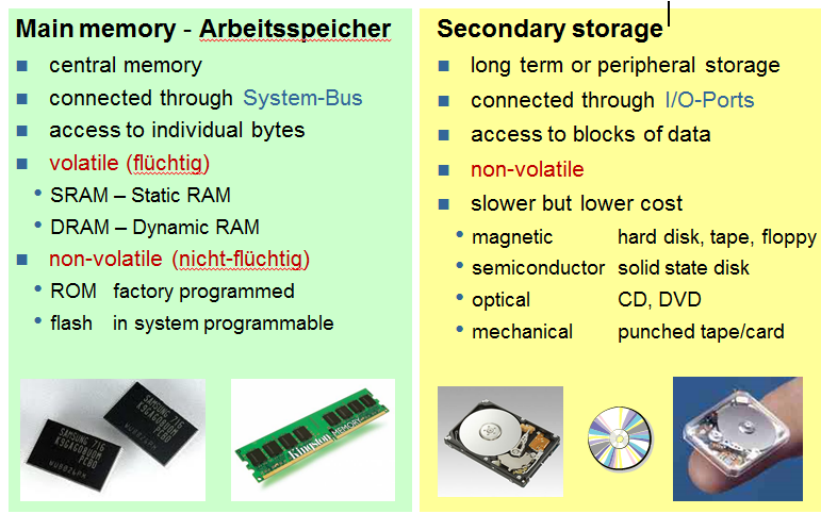
\includegraphics[width=\linewidth]{images/main_secondary_storage.png}
\end{example2}

\begin{example2}{Speichertypen zuordnen}\\
\begin{itemize}
  \item Flüchtig (volatile): Sekundärspeicher
  \item Nicht-flüchtig (non-volatile): Arbeitsspeicher
  \item Zugriff nur auf einzelne Bytes möglich: Arbeitsspeicher oder Sekundärspeicher
  \item Blockweiser Zugriff: Sekundärspeicher
\end{itemize}

\end{example2}

\begin{example2}{Memory Types and Organization}\\
Example of different memory access patterns:

\begin{lstlisting}[language=armasm, style=basesmol]
; RAM access example
    LDR     R0, =ram_data    ; Load RAM address
    LDR     R1, [R0]         ; Read from RAM
    
; ROM access example
    LDR     R0, =rom_const   ; Load ROM address
    LDR     R1, [R0]         ; Read from ROM
    
; Flash memory programming
    LDR     R0, =FLASH_BASE  ; Flash memory base
    LDR     R1, =0x12345678  ; Data to write
    ; Flash write sequence would go here
    
section_data
ram_data     SPACE   4       ; RAM variable
rom_const    DCD     0xFF    ; ROM constant
\end{lstlisting}
\end{example2}

\begin{KR}{Computer System Debugging}\\
Steps for debugging computer system issues:

1. Hardware level:
\begin{itemize}
  \item Check power and connections
  \item Verify clock signals
  \item Test memory access
  \item Check I/O interfaces
\end{itemize}

2. Software level:
\begin{lstlisting}[language=armasm, style=basesmol]
    ; Debug example
    PUSH    {R0-R3, LR}      ; Save registers
    BL      print_debug      ; Call debug routine
    ; Check specific values
    LDR     R0, =debug_var
    LDR     R1, [R0]
    CMP     R1, #expected
    BNE     error_handler
    POP     {R0-R3, PC}
\end{lstlisting}
\end{KR}

\begin{example2}{PC vs. Embedded System}\\
Erklären Sie den Unterschied zwischen einem Personal Computer (PC) und einem Embedded System bezüglich Aufbau, Anwendung und Programmausführung.\\
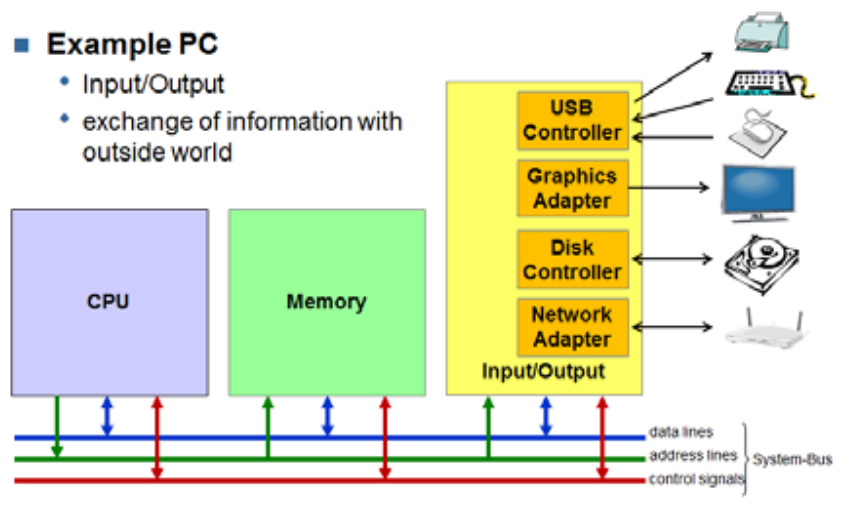
\includegraphics[width=\linewidth]{images/pcexample.png}

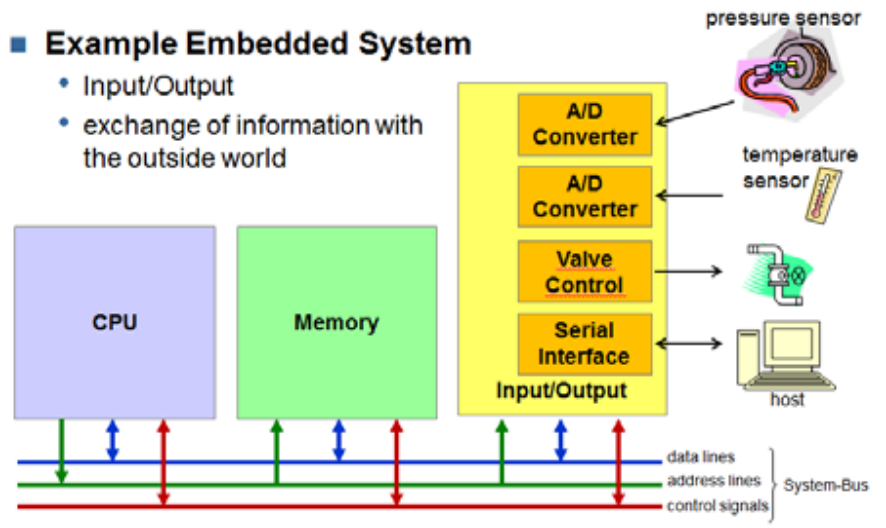
\includegraphics[width=\linewidth]{images/embeddedsystemexample.png}
\end{example2}



\begin{example2}{Wichtigkeit dieses Kurses}\\
Wieso ist Wissen um Assemblerprogrammierung wichtig?
\begin{itemize}
  \item Mit Hilfe von Assembler können wir verstehen, was auf der Maschinenebene abläuft 
  \item Verhalten von Programmen mit Fehlern besser verstehen
  \item Erhöhen der Performance:
  \begin{itemize}
    \item vorhandene und nicht vorhandene Optimierungen durch Compiler verstehen
    \item Ursachen für ineffiziente Programme finden und beheben
  \end{itemize}
  \item Implementieren von System Software: Boot Loader, Betriebssysteme, Interrupt Service Routinen 
  \item Lokalisieren und vermeiden von Sicherheitslücken (z.B. Buffer Overflows)
\end{itemize}
\end{example2}

